\documentclass[12pt, preprint]{hacked-aastex}
\usepackage{titlesec, hyperref, mdwlist, wrapfig, mdframed, enumitem}
\usepackage[style=numeric]{biblatex}

\bibliography{blanton}

\setlength{\topmargin}{0in}% 
\setlength{\headsep}{0in}% 
\setlength{\headheight}{0in}% 
\setlength{\textheight}{8.8in}% 

\newlength{\mylen}

\newenvironment{ditemize}
{ \begin{list}{}{%
\setlength{\topsep}{0pt}% 
\setlength{\partopsep}{3pt}% 
\setlength{\itemsep}{1pt}\setlength{\parsep}{1pt}% 
\setlength{\itemindent}{0pt}\setlength{\listparindent}{12pt}%
\setlength{\leftmargin}{24pt}\setlength{\rightmargin}{0in}%
\setlength{\labelsep}{3pt}\setlength{\labelwidth}{6pt}%
\setlength{\mylen}{3pt}
\renewcommand{\makelabel}{\makebox[\labelwidth][l]{\raisebox{\mylen}{\tiny$\bullet$}\hspace{\fill}}}}}
{\end{list}}


\begin{document}

\pagestyle{plain}
\titlespacing*{\section}{0pt}{0pt}{0.5\baselineskip}
\titlespacing*{\subsection}{0pt}{0.5\baselineskip}{0.5\baselineskip}
%\titleformat{\section}{\bfseries}{\thesection.}{1em}{} 

\newcommand{\imtxt}[1]{\textcolor{red}{#1}}
\newcommand{\imsout}[1]{\textcolor{red}{\sout{#1}}}

\title{{\large Characterizing the local population of mid-infrared-emitting active galactic nuclei}}

\maketitle

\renewcommand{\baselinestretch}{0.75}\normalsize
{\hypersetup{hidelinks} \tableofcontents }
\renewcommand{\baselinestretch}{1.0}\normalsize

% TODO
% - Connect Herschel, IRAS, GALEX

\newpage
\section{Summary}\label{sec:summary}

Unveiling the growth and development of galaxies is one of the ``prime
objectives'' of NASA's Cosmic Origins program.  Active galactic
nuclei, powered by accretion onto supermassive black holes at the
centers of galaxies, are thought to play an important role in the
evolution of galaxies by regulating and possibly quenching the
formation of stars.  For this reason, the Cosmic Origins program has a
focus on the history and evolution of supermassive black holes.  For
similar reasons, the National Academy of Sciences' Decadal Survey
report ``Pathways to Discovery in Astronomy and Astrophysics for the
2020s'' describes the study the growth of the supermassive black hole
population as essential to its priority science area, ``Unveiling the
Hidden Drivers of Galaxy Growth.''

We propose to characterize the population of mid-infrared (mid-IR)
emitting active galactic nuclei (AGN) and their host galaxies in the
local universe using data from the Wide-field Infrared Survey
Explorer, Spitzer Space Telescope, Herschel Space Observatory, IRAS,
and GALEX, combined with ground-based data from the Sloan Digital Sky
Survey IV (SDSS-IV; \cite{blanton17a}).  Our work builds on the
Mapping Nearby Galaxies at APO survey (MaNGA; \cite{bundy15a}), which
provides optical integral field spectroscopy for 10,000 galaxies at
redshifts $z<0.15$.  The ultraviolet and infrared data available from
the aforementioned NASA projects provides a powerful window into the
AGN population and the properties of the host galaxies.

Our work will advance the understanding of the mid-IR AGN population
in three ways. First, we will develop and test a new selection
criterion for mid-infrared AGN that promises to increase the AGN
sample by a factor of three and to extend the sample to lower
Eddington ratios. Second, we will carefully characterize the selection
effects and provide upper limits on mid-IR AGN luminosities. These
upper limits are essential to determining the distribution of AGN
properties as a function of galaxy host property, yet no previous
analyses have calculated them or accounted for them in analysis.
Third, by using the MaNGA sample as a basis we will be able to study
AGN host galaxy properties in unprecedented detail.

The primary results will be to measure the Eddington ratio
distribution as a function of host galaxy properties, and to
characterize the relationship between mid-IR AGN luminosities with
other AGN manifestations such as optical narrow lines and radio
emission. Galaxy formation simulations make direct predictions of the
relationship between AGN luminosity and galaxy properties and these
fundamental measurements will have the power to distinguish between
different theoretical models. The relationship between galaxy
properties, mid-IR AGN emission, and other manifestations of AGN can
be used to understand the fundamental structure of the central gas and
dust structure (the ``torus'') in AGN.

This work therefore will provide new results of fundamental importance
to understanding the nature of supermassive black hole accretion and
its effects on galaxy evolution, using the AGN in the universe whose
galaxy host properties we can measure the best.

%\newpage
\section{Objectives \& Relevance: AGN and Galaxy Evolution}\label{sec:intro}

\fbox{\parbox{\textwidth}{\bf This proposed work will establish a new 
low redshift baseline for the distribution of AGN properties
that galaxy formation theorists can use as a new observational 
constraint. In this section we explain the theoretical context 
that makes this work significant and important.}}

A central question in galaxy formation is why the most massive
galaxies have not converted more of their available baryons into
stars, and instead have ended their star formation. This question has
existed in some form or other since at least the work of
\cite{white78a}, when the first models of galaxy formation inside of
dark matter halos predicted highly efficient cooling of gas. As
$N$-body and hydrodynamic simulations became more sophisticated this
problem shifted in many details but essentially remained the same: the
halo mass function extends nearly as a power law to high masses,
whereas the galaxy stellar mass function cuts off as nearly an
exponential.  A straightforward application of gas cooling physics to
cosmological hydrodynamic simulations predicts that the stellar mass
function should more closely follow the halo mass function, and 
\cite{benson03a, somerville15a}.

Many solutions have been considered, and under the right set of
assumptions several of them are tenable, but the most commonly held
assumption is that the tremendous energy output by AGN in massive
galaxies is implicated somehow in heating and possibly driving out the
gas, preventing excessive star formation.

This solution has several attractions, summarized in
\cite{fabian12}. The AGN are highly efficient generators of energy for
heating and winds, which are indeed observed to be acting in a number
of cases. Back-of-the-envelope calculations suggest that AGN-produced
radiation pressure on dust in gas can act as negative feedback
naturally limiting accretion onto a galaxy. The $M_{\rm BH}$--$\sigma$
relation appears to point to some sort of co-evolution of galaxies and
their black holes. Finally, only with AGN feedback can hydrodynamic
simulations reproduce key observables: the fractions of quenched
massive galaxies found in isolation and the stellar mass function
itself \cite{somerville15a, wellons22a}.

This situation, however, is not ``case closed.'' The hydrodynamic
simulations:
\begin{itemize}
\item Each have their AGN feedback and other parameters tuned to fit
  certain observations; to show whether the model is actually correct,
  we need to test additional predictions;
\item Each have different, sometimes dramatically different, methods
  for applying AGN feedback, which yield different relationships
  between AGN activity and galaxy properties.
\end{itemize}
So which of these various theories of AGN feedback (if any) describes
the real universe? An important prediction we intend to test is what
they predict about the population of AGN in galaxies today.

In detail, the simulations cannot follow black hole seeding, growth,
and AGN feedback from first principles. These processes all are
governed by physics on orders of magnitude smaller scales than the
simulation resolution, so require subgrid prescriptions.  Generally
black hole growth is modeled with Bondi-Hoyle-Lyttleton accretion
\cite{edgar04a}, but with details varying between simulations. The
accretion model determines the accretion rate, which is often
expressed as the Eddington ratio $\lambda$ between the actual rate and
the Eddington rate, the maximum rate for spherical accretion onto a
black hole of a given mass.

The feedback prescriptions vary more widely. There are two basic types
of feedback implemented: thermal feedback (i.e. inserting thermal
energy into the gas surrounding the black halos) and kinetic feedback
(inserting momentum into the gas surrounding the black holes).  Table
\ref{table:feedback} summarizes how these are used.  Some simulations
use one of these types, some use the other, and some use both, with
the choice dependent on the Eddington ratio $\lambda$. IllustrisTNG
and Horizon-AGN use the most ``natural'' choices: the high $\lambda$
mode uses thermal feedback, which best corresponds to the
observational radiative/thermal/quasar mode, and the low $\lambda$
mode uses kinetic feedback, which best corresponds to the
observational kinetic/jet/radio mode. IllustrisTNG uses an extra
dimension of parametric freedom to allow the Eddington ratio division
between these modes to vary with black hole mass.  In cases like SIMBA
and Illustris, although the basic type of feedback is unchanged, the
exact implementation does change between low and high accretion.

These various refinements of the AGN feedback methodology have been
designed to best recover galaxy properties. All of the simulations
recover basic scaling relations and demographics of galaxies
reasonably well, though many of these methods still struggle to fully
quench the most massive galaxies.


\begin{table}[t!]
\caption{\label{table:feedback} 
AGN Feedback Methods In Cosmological Simulations\\ ~}
\begin{tabular}{|c|c|c|c|}
\hline
Simulation & Eddington Ratio Criterion & High $\lambda$ Mode & Low $\lambda$ Mode \cr
\hline
\hline
Illustris \cite{sijacki15a} & 0.05 & Thermal & Thermal \cr
IllustrisTNG \cite{weinberger17a} & 0.002---0.1 & Thermal & Kinetic \cr
Horizon-AGN \cite{dubois14a} & 0.01 & Thermal & Kinetic \cr
SIMBA \cite{dave19a} & 0.2 & Kinetic & Kinetic \cr
EAGLE \cite{schaye15a} & --- & \multicolumn{2}{c|}{Thermal} \cr
NIHAO \cite{blank19a} & --- & \multicolumn{2}{c|}{Thermal} \cr
\hline
\end{tabular}
\end{table}

The investigation of \cite{habouzit22a} shows that these predictions
vary dramatically in Eddington ratio distributions and their
dependence on galaxy properties, particularly on stellar mass. For
example, some of the Eddington ratio distributions increase with mass,
some decrease, some are non-monotonic.  These differences between the
simulations' predictions for the Eddington ratio distribution as a
function of host galaxy properties provide a critical test of galaxy
formation models.

Note that the work of \cite{habouzit22a} also underscores some of the
difficulties of this prediction and its comparison to observations.
The AGN accretion and feedback models need to be converted into some
estimate of observables. The AGN observables are X-ray luminosity,
broad line emission, narrow line emission, IR emission, and radio
emission. The X-ray and optical line emission (particularly the broad
line emission) is further modified by dust obscuration in the
surroundings of the AGN, which cannot directly be predicted from the
simulations. These difficulties motivate the better observational
understanding the joint distribution of these multiwavelength
signatures of AGN.

Currently the statistical distribution of AGN luminosities as a
function of galaxy properties is poorly understood, both because of a
relative paucity of mid-IR AGN with well-measured galaxy host
properties and because the selection effects on the existing samples
have not been well characterized.  In this work, we propose to unveil
a larger population of mid-infrared emitting AGN than it was
previously possible to reliably detect, and to also set accurate upper
limits on mid-IR AGN emission for galaxies without detected AGN. From
these measurements we can determine the luminosity and Eddington ratio
distributions of AGN as a function of galaxy properties.  These
observations will establish an important new low redshift constraint
on galaxy formation simulations.

\section{Scientific Impacts: AGN host galaxies and Eddington ratio distributions}\label{sec:intro}

\fbox{\parbox{\textwidth}{\bf This work is part of our effort to 
establish more firmly the relationship between AGN properties 
and their host galaxies in the  local universe. In this section, 
we explain how this work advances  the state of the art, and what 
the specific  measurements we intend to make are.}}

The major goal of our group's work---of which this proposal is one
part---is to constrain the distribution of AGN luminosities as probed
in many ways (e.g. radio, infrared, optical narrow lines, and X-rays)
as a function of stellar mass $M_\ast$, velocity dispersion
$\sigma_v$, and star formation rate (SFR):
\begin{equation}
\label{eq:model}
\Phi\left(L_{\rm radio}, L_{\rm IR}, L_{\rm OIII}, L_X | M_\ast, \sigma_v, {\rm SFR}\right),
\end{equation}
Surprisingly, observational constraints on this distribution are not
as well-understood as they could be, and much of the literature on the
subject is riddled with difficult-to-understand selection effects 
(see \cite{trump15a} for a description of the selection effects 
on optical narrow line AGN, for example).

The underlying problem is that AGN manifest in a variety of different
ways, depending both on their intrinsic state and on the viewing angle
of the observer, and across all wavelengths of light.  To make things
more complicated, their signatures are often in competition with
stellar emission and interstellar gas emission. 

But the understanding of the AGN distribution is further hampered by 
the  way that it is typically studied. Most AGN demographic 
focus on identifying AGN (\cite{kauffmann03b, lacy15a, sanchez19a, 
comerford20a, greene20a}) 
but {\it do not}  determine the upper limits on luminosity caused by
effects of host galaxy contamination 
(\cite{trump15a, jones17a} being rare exceptions). This approach clearly 
throws out important information, and also makes the resulting analyses 
susceptible to  untracked selection effects. It makes it impossible
to study the population of low luminosity AGN accurately, since whether
a given low luminosity AGN is identifiable largely depends on the
host galaxy properties.

In this work we propose to advance the understanding of the
distribution of infrared AGN luminosities $L_{\rm IR}$ and 
Eddington ratios, and its dependence on host galaxy properties,
at low redshifts.  We will measure the mid-IR
AGN-related luminosities for detected AGN {\it and} upper limits for
galaxies without detected AGN. We will create a new, larger sample
and probe lower luminosity and Eddington ratio AGN than were
previously identified in low redshift samples.

{\bf New and archival observations of the low redshift universe
  present an opportunity to make progress on these
  questions}. Specific motivations for revisiting this question are:
\begin{ditemize}
\item With the Sloan Digital Sky Survey's Mapping Nearby Galaxies at
  APO (MaNGA) program, we can measure low redshift galaxies
  exquisitely well, and separate spatially the AGN and galaxy emission
  (\cite{bundy15a, blanton17a}).  Our analysis takes advantage of
  10,000 potential AGN host galaxies from MaNGA with high
  signal-to-noise ratio measurements of stellar mass, velocity
  dispersion, SFR, and other parameters.
\item Existing surveys in the infrared (IR) from the Wide-field
  Infrared Survey Explorer (WISE; \cite{wright10a}) are well matched
  to find mid-IR AGN in MaNGA galaxies \cite{comerford20a}. But
  previous searches for AGN in WISE have focused on the most extreme
  AGN, whereas lower Eddington ratio AGN are readily identifiable but
  have not been studied previously.
\item The Spitzer Space Telescope archive has mid-IR spectroscopy of
  galaxies in MaNGA and other nearby galaxies, which we can use to
  validate the lower Eddington ratio cases and to study more detailed
  properties of the mid-IR emission.
\end{ditemize}

The well-measured MaNGA host galaxy properties present a unique
opportunity relative to most other AGN samples.  The mid-IR-based
bolometric luminosity distribution of AGN and its evolution has been
measured by massive samples of AGN selected in the mid-IR
\cite{lacy15a}. However, it is ambiguous how these AGN relate to their
underlying host galaxies and the black holes themselves, because for
these samples relatively little can be inferred about their host
galaxies.  The galaxies tend to be faint, higher redshift, outshone in
many cases by their AGN, and poorly resolved.  This lack of
information also makes it difficult to account for systematic
differences between low mass and high mass galaxies in selecting AGN;
star formation in low mass galaxies may be more easily confused with
AGN because they are lower metallicity and consequently have less PAH
emission and hotter dust \cite{hainline16a, sajina22a}.

In this work, we will utilize these new resources to answer the
critical question of how AGN populate host galaxies in the low
redshift universe. {\bf The direct impact of this work will be to}:

\fbox{
\begin{minipage}{0.9\textwidth}
\begin{ditemize}
    \item Expand the potential sample of mid-IR emitting AGN in the
      local universe by a factor of three, and extending to lower
      Eddington ratios and luminosities, by validating a new selection
      technique.
    \item Provide observational constraints on galaxy formation theory
      from the Eddington ratio distribution of mid-IR emitting AGN as
      a function of stellar mass, velocity dispersion, and star
      formation rate.
    \item Explore the relationship between different manifestations of
      AGN (optical narrow line, X-ray, ratio, mid-IR) as a function of
      host galaxy properties.
\end{ditemize}
\end{minipage}
}

This work will have long term indirect impacts as well. The
well-validated selection function we develop will be
applicable for use in larger samples (with less information per
galaxy) such as the SDSS Legacy Survey and the DESI Bright Galaxy
Survey. Doing so would massively increase the power of the legacy WISE
data set for the purposes of selecting AGN in the local and more distant
universe.

\section{Methods of Proposed Work\label{sec:methods}}

To achieve the goals laid out above to advance our understanding 
of AGN in the local universe, we use the following methods;
\begin{ditemize}
    \item We use a low redshift sample of galaxies from MaNGA with 
    jointly analyzed WISE data (the MaNGA NASA Sloan Atlas or MNSA)
    (Section \ref{sec:mnsa}).
    \item We use a newly developed, more sensitive criterion to 
    identify AGN  (Section \ref{sec:criterion}).
    \item We use SED modeling methods to derive the mid-infrared AGN 
    luminosities and upper limits for all 10,000 MaNGA galaxies
    (Section \ref{sec:measurements}). 
    \item We analyze Spitzer Space Telescope spectra to validate our 
    classifications and measurements of mid-IR (Section
    \ref{sec:spitzer}).
    \item We perform a maximum likelihood analysis using mid-IR AGN luminosities 
     and upper limits to constrain the Eddington ratio  distribution as a 
     function of galaxy properties (Section \ref{sec:erd}).
    \item We compare the mid-IR AGN luminosity distribution to other manifestations 
    of AGN in this sample (Section \ref{sec:other}).
\end{ditemize}

\subsection{The MaNGA NASA Sloan Atlas}
\label{sec:mnsa}

MaNGA comprises the best understood sample of 10,000 galaxies in the
universe, with comprehensive integral field spectroscopy in the
optical, constraining galaxies' central velocity dispersion, star
formation history, ionized gas properties, and dynamics. WISE
photometry detects every MaNGA galaxy and provides important
information about their AGN and star formation activity that we will
make use of here. We will make use here of a combination of GALEX,
MaNGA, and WISE data created in previous research, called the MaNGA
NASA Sloan Atlas (MNSA).

The MaNGA measurements provide an immense amount of ancillary
information, unparalleled in any other sample of its size, and we do
not need to perform analysis with this grant to extract this
information, but can rely on already-published analyses.  MaNGA
spectroscopy extends out to at least 1.5$R_e$ for every observed
galaxy, allowing inference of reliable stellar masses and star
formation rates from stellar population analysis \cite{sanchez22a},
dynamics (e.g. \cite{graham18a}), ionized gas properties (e.g.,
\cite{belfiore17a}), and many other properties.  These galaxies have a
median redshift of $z\sim0.03$, with the sample extending out to
$z\sim 0.15$, and the physical spatial resolution is typically around
1--2 kpc. They have been selected in a well-defined way as a function
of mass and color, so that each MaNGA Main Sample galaxy's relative
probability of having been observed is known, making the sample
suitable for statistical study \cite{wake17a}.

This sample has some important advantages for conducting a statistical
study of AGN with low redshift galaxies.  Star formation rates over
the past 100 Myrs can be inferred from the stellar population
analysis, which avoids dependence on the H$\alpha$ emission, which
could be contaminated by the presence of an AGN.  The high
signal-to-noise ratio stellar velocity dispersion maps can provide an
estimate of the central black hole using the $M_{\rm BH}$-$\sigma$
relationship \cite{kormendy04b}. The narrow line measurements allow us
to find nuclear narrow line regions as well as extended narrow line
regions and outflows. The sample is low enough redshift that
essentially every galaxy has informative detections in WISE.

Because we start with a galaxy sample with a well-understood
selection, we can also use this sample for accurate AGN population
measurements, for example constraints on the Eddington ratio
distribution as a function of galaxy mass, star formation rate,
metallicity, or other properties.  As argued by \cite{aird12a} in the
context of X-ray selection, this situation contrasts with samples {\it
  selected} on their AGN-ness, for which the host galaxy properties
are biased at best but often inaccessible entirely.

In previous work we have performed careful photometry from GALEX and
WISE images for all MaNGA galaxies, and created ultraviolet, optical,
and mid-infrared images on a common sampling. The resulting MNSA
catalog will be the basis of our work here.

\subsection{Identifying AGN in WISE: A New Criterion}
\label{sec:criterion}

We use the W1, W2, and W3 bands, along with the star formation rates
and gas-phase metallicities determined for MaNGA galaxies, to identify
mid-IR emitting AGN, to estimate their luminosities (accounting for
the contribution of star formation), and to estimate upper limits on
the mid-IR AGN luminosities for galaxies without detections. {\bf 
We propose to test and use a more inclusive criteron that promises
to provide around a factor of three more AGN than the previous 
standard criteria.}

AGN often manifest with mid-IR emission from dust in the periphery of
the accretion disk heated to close to sublimation temperatures,
considerably hotter than dust temperatures in star forming regions.
The W1$-$W2 color (i.e. the 4.6 $\mu$m to 3.4 $\mu$m flux ratio) is
sensitive to this AGN emission because stellar populations have a
roughly uniform W1$-$W2 color (those bands are in the
Rayleigh-Jeans regime).  Meanwhile, dust heated by star formation does
not get to high enough temperature to contribute much to W2, nor do
most PAH lines.  The W1$-$W2 color of a star forming host can be
inferred from its star formation rate (or from its W2$-$W3 color).
Therefore, a W1$-$W2 color redder than that predicted from its star
formation history suggests the presence of hot dust indicative of an
AGN.

Figure \ref{fig:wise} illustrates these effects, showing the
relationship between this color and the specific SFR (sSFR) of MaNGA 
galaxies from \cite{sanchez22a}.  At low W1$-$W2, there is a tight sequence
of points with a clear sSFR dependence; for these galaxies, both bands
are dominated by the host galaxy.  For the reasons described above,
the presence of an AGN and its attendant hot dust leads to redder
W1$-$W2, and the ``spray'' of points above the tight sequence are
likely to be AGN. 

\begin{figure}[t!]
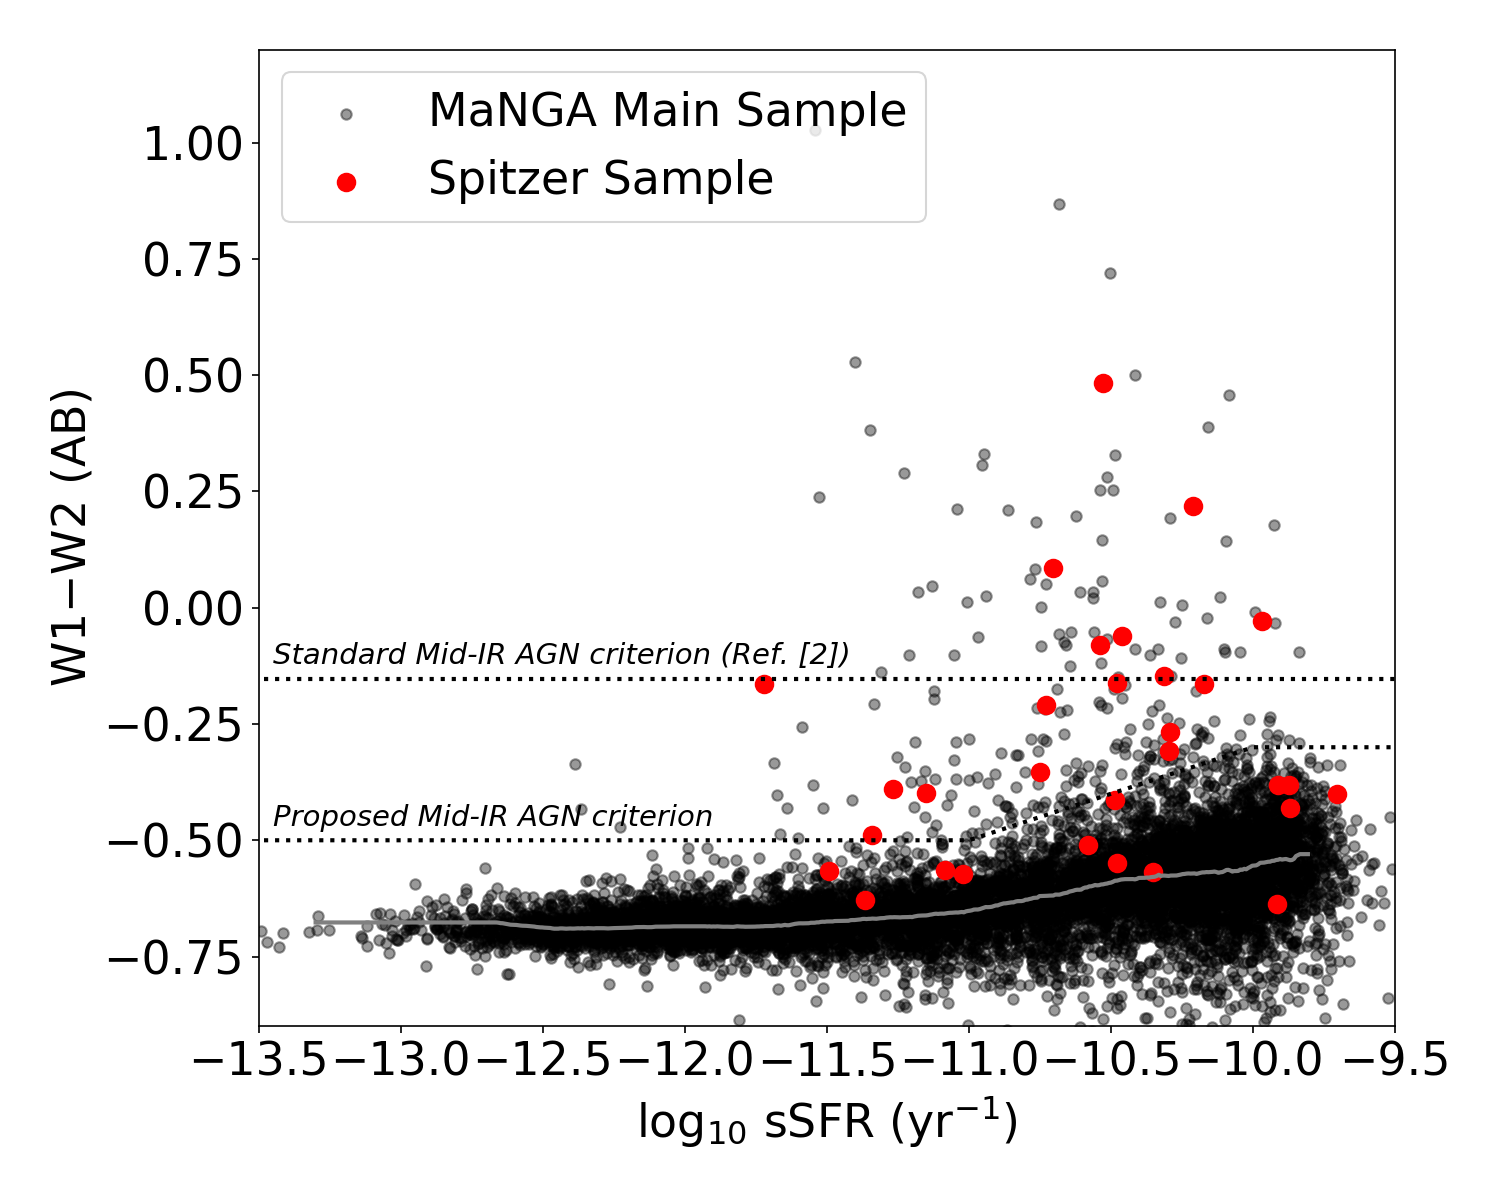
\includegraphics[width=0.64\textwidth]{w1w2-vs-ssfr.png}
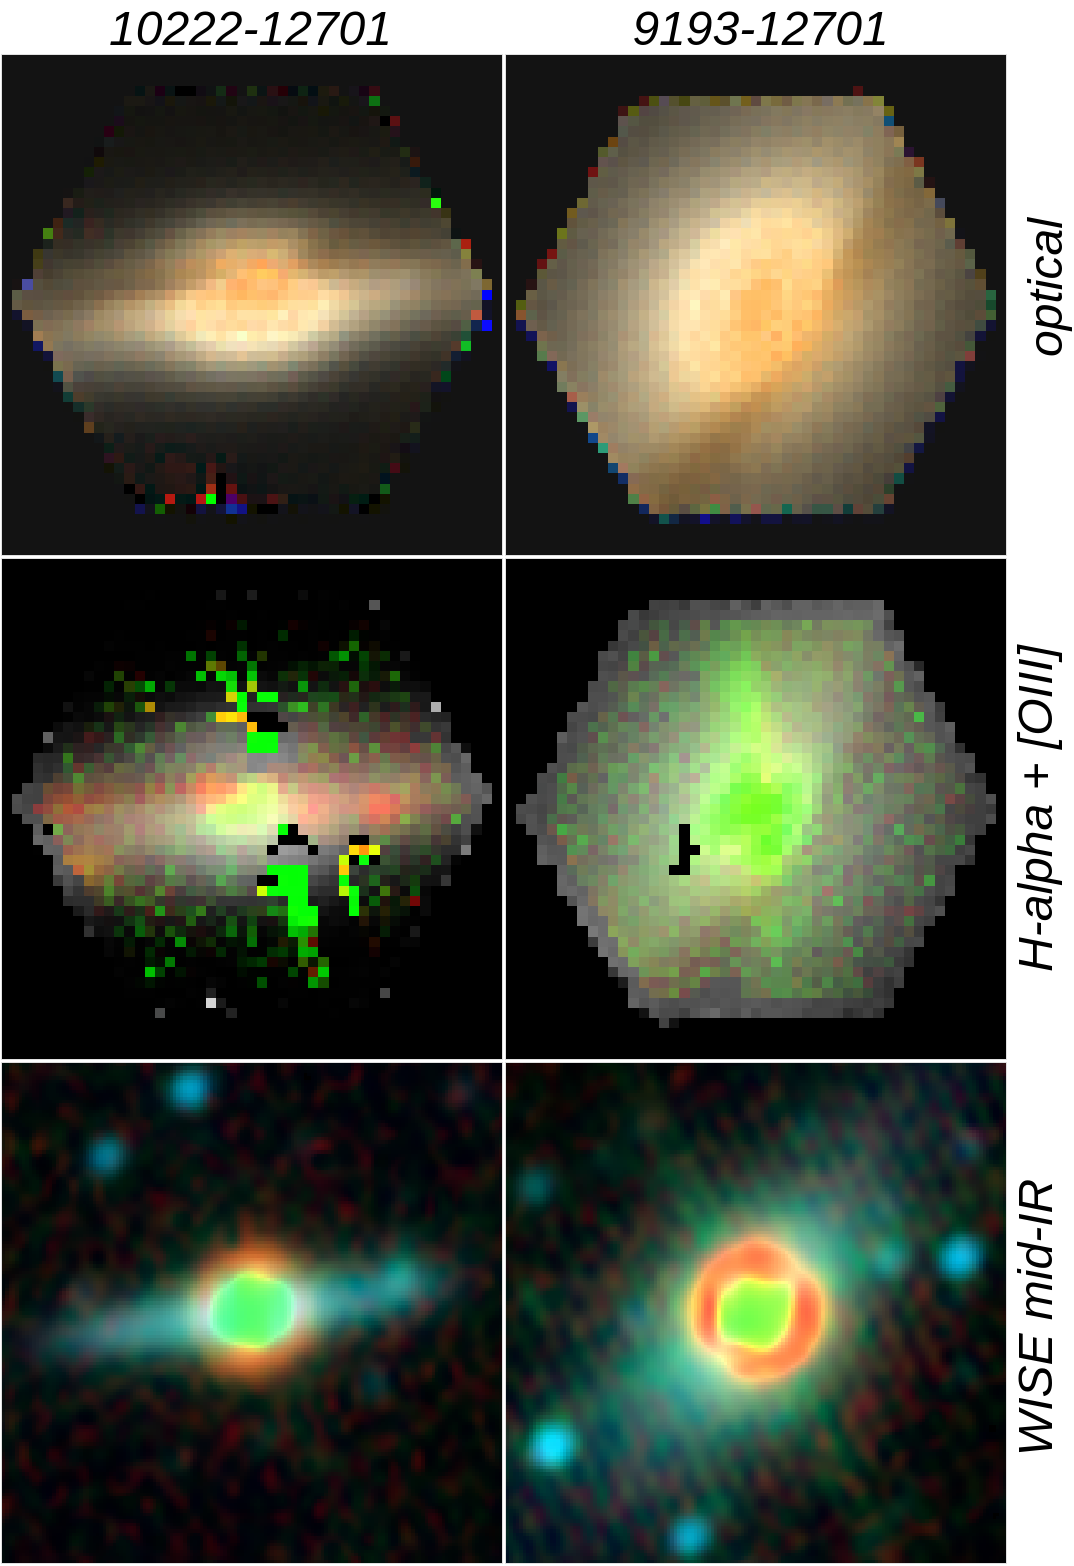
\includegraphics[width=0.35\textwidth]{ir-grid.drawio.png}
  \vspace{-22pt}
    \caption{
\label{fig:wise} \small Mid-IR AGN detection. 
The left panel shows W1$-$W2 colors (AB) of MaNGA galaxies vs star
formation rate determined from the optical stellar population fits.
The dotted line is the commonly used AGN criteria from
\cite{assef18a}. The grey line is designed to follow the dependence
of W1$-$W2 on SFR, and (with care taken to validate it) will provide
a more complete census of IR AGN from the MaNGA sample. The right
panel shows two example AGN selected in the mid-IR, with one that
only passes the proposed new criterion and one that passes both 
criteria. The top shows the optical broadband color image; the middle shows 
the optical broadband light as grey, with [OIII] emission overlaid
as green and H$\alpha$ emission overlaid as red; the bottom shows
the WISE mid-IR color image. Notably, the newly included galaxy
is clearly an AGN from its [OIII] emission and morphology.}
\end{figure}

The upper dotted line shows the typical criterion used to select AGN
(specifically, the most inclusive criterion from from \cite{assef18a},
here translated to AB magnitudes). However, there are many objects in
between this criterion and the sequence of non-AGN. The reason that
\cite{assef18a} and almost all other references choose such conservative
criteria even in their most inclusive samples is that typically they
do not know much about the host galaxy properties.  The vast majority
of WISE-detected AGN do not have a redshift and therefore no
appropriate $K$-correction. The observed-frame W1$-$W2 colors, without
any known host galaxy color to compare to, is much less informative
and therefore the criterion used must be much more
conservative. Alternative criteria to those in \cite{assef18a} are
all more conservative than the one shown in Figure \ref{fig:wise} and
therefore include even fewer candidates \cite{jarrett11a,stern12a}, 
except for that of \cite{hviding22a}.

For the MaNGA-based sample, we do not have these 
difficulties. We can define a criterion that hews more tightly 
to the intrinsic host galaxy distribution, defined by the lower 
dotted line. This new criterion increases the mid-IR emitting AGN 
candidate sample by a factor of three.

We will examine the degree to which other galaxy information,
such as stellar metallicity, stellar mass, velocity dispersion,
or Balmer decrement, correlate with the scatter around the grey line in 
Figure \ref{fig:wise} and therefore help predict the host galaxy
W1$-$W2. The work of \cite{hviding22a} (see above) shows a similar
pattern as seen in Figure \ref{fig:wise} but with W2$-$W3 replacing
sSFR, and also propose defining a more agressive color cut than
\cite{assef18a}; we 
will investigate the extent to which this color can provide 
additional information.

\subsection{Measuring mid-IR AGN luminosities and upper limits}
\label{sec:measurements}

For every galaxy in this sample we seek to produce either: (a) a
measured mid-IR AGN luminosity or (b) an upper limit on the mid-IR AGN
luminosity, if an AGN is not detected. For every identified AGN we
will infer a 6 $\mu$m luminosity using an SED-based analysis of the
photometry. For every galaxy without an identified AGN, we will
determine using a typical AGN SED what 6 $\mu$m luminosity it would
have to have had in order to be classified as an AGN, placing thereby
an upper limit on that luminosity. {\bf Previous work with mid-IR AGN
  from WISE has neither accounted for the host galaxy contribution in
  the determination mid-IR luminosity or in calculations of upper
  limits in mid-IR luminosity; we do so here with the use of SED
  fitting techniques}.

Even for the extreme mid-IR AGN selected by \cite{assef18a}, their
W1$-$W2 values are only 0.5--2 mag redder than the host galaxy
sequence. Thus, a considerable fraction---more than half in some
cases---of the W2 luminosity is from the host galaxy itself. It is
therefore essential to account for the contamination due to the host
galaxy. For this reason previous work such as \cite{hviding22a} have
not calculated mid-IR-based luminosities for objects like those
we are interested in.  

We can crudely estimate the mid-IR AGN luminosity in W2 by using the
excess W1$-$W2 over the grey line in Figure \ref{fig:wise}.  If we
assume the entire excess is due to the AGN contribution to W2, and
that it makes no contribution to W1, we can infer the AGN contribution
to W2. We then can convert that W2 flux to a 6 $\mu$m luminosity using
the AGN SED from \cite{richards06a} or from one of the typical AGN
SEDs that we fit below from \cite{nenkova08a}.  Similarly, we can
calculate a crude estimate of an upper limit on the AGN luminosity by
using the difference between the grey line and our color criterion for
the sSFR of any particular galaxy; this will tell us how much AGN
luminosity would be necessary to classify that galaxy as an AGN.
These crude estimates have the virtues of simplicity and model
independence.

But more precise estimates of the AGN mid-IR luminosity and upper
limits can be made using SED fits including AGN and star formation
components. We will use a non-negative fit to a large set of stellar
population templates from the Flexible Stellar Population Synthesis
models (FSPS; \cite{conroy09a}), along with a set of AGN templates
from the ``Clumpy'' models \cite{nenkova08a}.  Performed with a Python
version of the {\tt kcorrect} software \cite{blanton07a}, these fits
are extremely fast, taking a fraction of a second per galaxy.

A preliminary example of one of these fits can be seen in Figure
\ref{fig:fits}. This figure illustrates two points: (a) how the AGN
dust emission reddens the W1$-$W2 color, and (b) that the AGN can be
clearly detectable while being a minority contributor to the W2
flux.

We will characterize the luminosity of the AGN component at several
wavelengths, concentrating primarily on 6 $\mu$m and 15 $\mu$m, 
commonly used reference points. We will use our error analysis (see 
below) to determine which wavelengths are most strongly constrained
in the presence of modeling uncertainty and thus most suitable for 
bolometric luminosity estimates. 

For the MaNGA sample of bright galaxies, we anticipate that the 
15 $\mu$m luminosity will be much better measured and less 
contaminated by the host galaxy.
But for larger, deeper samples that are based on  WISE 
\cite{assef18a, hviding22a}, we anticipate that W3 and W4 
will not be well enough measured for good constraints on 15 $\mu$m.
With this in mind, we will determine the relationship 
between the 6 $\mu$m and 15 $\mu$m AGN luminosities within MaNGA,
so that that relationship can be used to bootstrap 6 $\mu$m 
measurements made with larger samples.

\begin{figure}[t!]
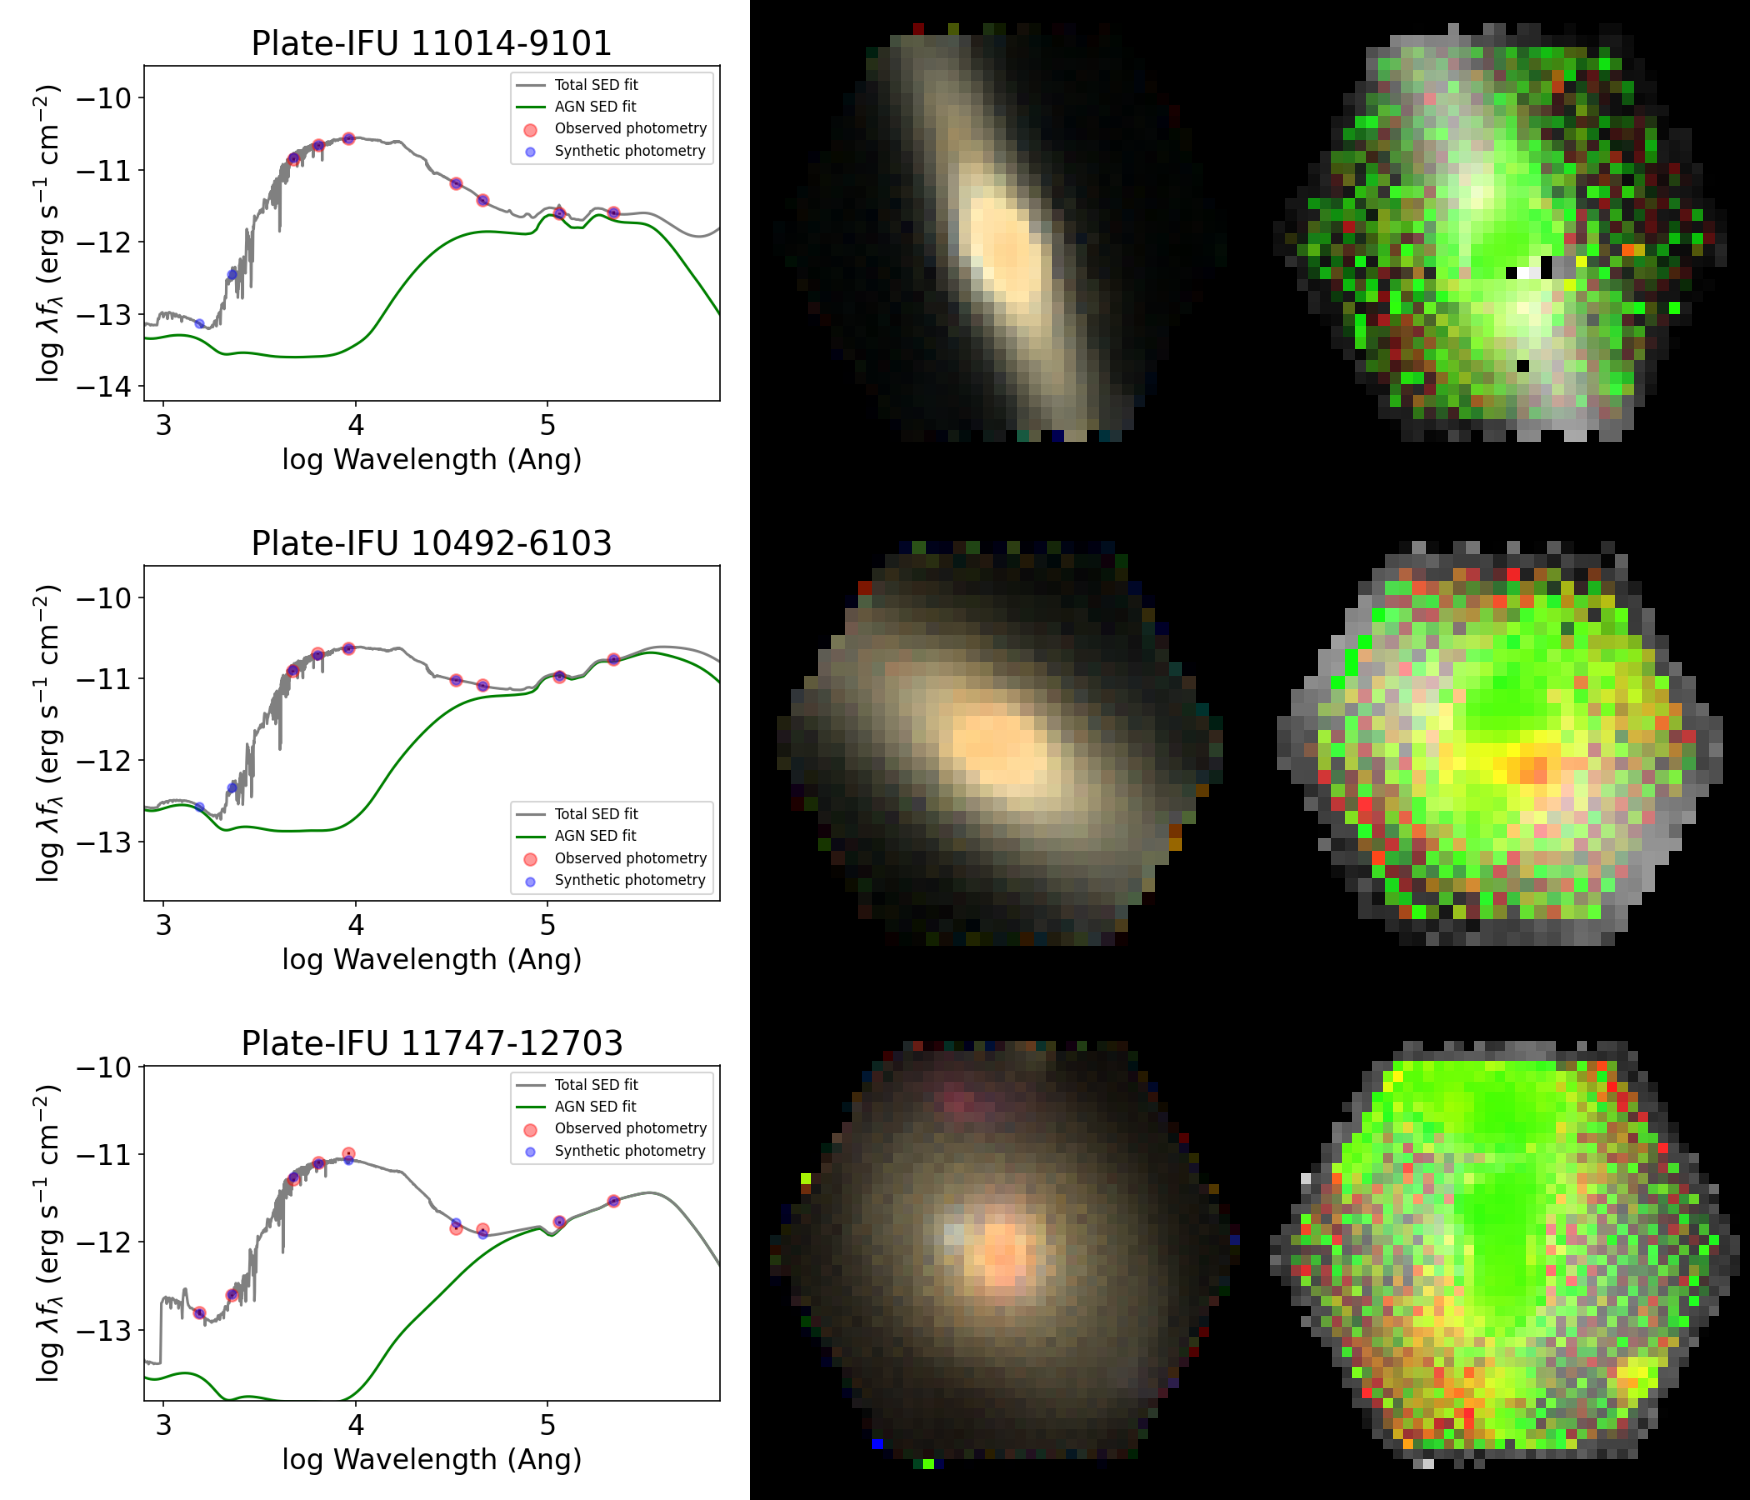
\includegraphics[width=0.98\textwidth]{spec-grid.png}
    \caption{
\label{fig:fits} \small SED fits to identified AGN. Each row
corresponds to a mid-IR detected AGN. On the left is shown the
broad-band photometry along with our preliminary SED fits.  The grey
line shows the total SED including the stellar populations, emission
lines, dust emission from the ISM, and AGN emission. The green line
just shows the contribution from AGN. The models show that AGN
contribution in the mid-IR needs to account for the stellar
contributions. On the right are the broad-band color and emission line
images from MaNGA as described in Figure \ref{fig:wise}.}
\end{figure}

The use of the SED fitting techniques makes it straightforward to
calculate uncertainties and upper limits. We will perform a large set
of Monte Carlos on the data set, adding random errors to the fluxes
based on the measurement uncertainties. The resulting distribution of
Monte Carlo AGN luminosities provides an estimate of the errors, that
accounts for the statistical errors and for the wide variation
possible in the AGN and stellar population models. For identified AGN,
these results determine the luminosity errors.

For galaxies without identified AGN, we can use the best fit SED to
help determine the upper limit. First, we will determine a ``typical''
AGN SED from the fits to galaxies with mid-IR AGN; we will also
determine this typical AGN SED as a function of sSFR to test for
systematic variations. Second, for each galaxy without an identified
AGN we can determine how much typical AGN SED can be added to its
best fit SED before it crosses our color threshold for AGN. The combined
AGN luminosity from both components evaluated at 6 $\mu$m is our 
estimate of the upper limit.

There are inherent uncertainties in the SED fitting process related
to our understanding of the SED models. We will explore the
effects of varying the AGN and stellar population SED grids on our
results to test their robustness.  As described in the next section,
we will further test this fitting procedure with the detailed spectra
from Spitzer. The testing procedure may lead to adjustments in the
underlying grid of SED models we use for the full set of galaxies.

%Eddington ratio about 0.6 dex lower than the standard AGN as selected
%by \cite{assef18a}.

\subsection{Analysis of Spitzer Space Telescope Spectra}
\label{sec:spitzer}

With only broad-band WISE fluxes, there will be uncertainties in the
population of AGN unveiled with our new criterion, both in the AGN
identification and in the measurement of luminosity. To address these
uncertainties, we will make use of around 2,000 Spitzer Space
Telescope spectra in the mid-IR compiled by \cite{lambrides}. Of this
sample, 30 are in our MaNGA sample and can provide direct tests.
Figure \ref{fig:spitzer} shows several examples of these spectra.  Our
technique will be to use traditional signatures and the shape of the
spectrum to inform our interpretation of the WISE photometry.

We will examine the relationship between W1$-$W2 and traditional
signatures such as the PAH 6.2 $\mu$m equivalent width. The PAH
measurement is strong if the galaxy is dominated by star formation,
but weak if the emission is dominated by the AGN \cite{sajina22a}.
For the full sample of 2,000 spectra from \cite{lambrides}, we will
use strong PAH signatures to estimate the outlier rate as a function
of W1$-$W2.  The 40 galaxies with MaNGA data and Spitzer spectra will
provide less statistically powerful but more detailed information. In
these cases, we can use MaNGA-based information on the gas metallicity
to control for the PAH strength dependence on metallicity.

{\bf also talk about silicon feature}

We will assess and refine our SED fitting with the Spitzer spectra as
well.  In the case of the 40 galaxies with MaNGA and Spitzer data, we
can directly compare the SED fitting results for the broad-band
photometry to the detailed Spitzer spectra and assess its
validity. For the other Spitzer spectra, we will fit using our models
to synthesized photometry and then assess the results similarly. We
will use the differences in broad-band spectral shape and in the
prominence of the PAH lines to refine our choice of FSPS and AGN
template parameters to better reflect the more detailed Spitzer
spectra.

For a small number of the Spitzer spectra, we can also examine other
AGN indicators. The spectra show high ionization lines, in particular
[Ne V] 14.3 $\mu$m, [S IV] 10.5 $\mu$m, [O IV] 26 $\mu$m, which we
expect to be good tracers of AGN activity and can be used to validate
the existence of a strong AGN.

\subsection{Fitting Eddington Ratio Distributions}
\label{sec:erd}

The primary observational results we seek are the mid-IR luminosity
and Eddington ratio distributions as a function of galaxy properties,
in particular stellar mass ($M_\ast$), velocity dispersion ($\sigma$),
and specific star formation rate (sSFR).

We will calculate the mid-IR luminosity distributions using a standard
maximum likelihood technique utilizing the mid-IR luminosities and
upper limits observed for the sample. Specifically, we seek the
quantity:
\begin{equation}
\Phi\left(L_{\rm IR} | X\right)
\end{equation}
where $X$ is $M_\ast$, $\sigma$, or sSFR. The advantage of the MaNGA
sample is that these quantities are known extremely reliably. We will
use at least two choices of parametrization---a broken power law and a
Schechter function. Given the limitations in sample size, we expect
that we will not be able to determine the full joint dependence on
multiple properties. Instead, for each choice of $X$ we will search
for residual dependence on the other two properties. Within any given
model, we will maximize the log-likelihood, which can be expressed as:
\begin{equation}
\ln \mathcal{L} \propto 
\end{equation}
which utilizes both the mid-IR AGN detections and the upper
limits. The upper limits are critical for this study since they allow
us to utilize the many non-detections, which can be quite informative
about the fraction of galaxies with low luminosity AGN when used
properly.

To calculate Eddington ratios we need to infer both the bolometric
luminosity and the black hole mass (which sets the limiting Eddington
luminosity). In our context, the absolute level of the Eddington ratio
is less important than that we provide some appropriate scaling of the
AGN emission as a function of black hole mass.  For the bolometric
luminosity we will use the nonlinear relation of \cite{stern15a}
between mid-IR luminosity and X-ray luminosity, and assume a factor of
20 between X-ray luminosity and bolometric luminosity. Although this
approach is susceptible to variations in the bolometric-to-mid-IR
luminosity ratio, we note that the sample we develop will be well
matched to future public eROSITA catalogs, in order to help better
calibrate this relationship.

We will infer the black hole mass using the central velocity
dispersion from the MaNGA data and the $M_{\rm BH}$--$\sigma$
relation, which is measured at high precision.  A major advantage of
our sample relative to others (particularly larger but lower
signal-to-noise ratio samples like SDSS Legacy and the upcoming DESI
Bright Galaxy Survey) is the excellent measurements of $\sigma$ of the
host galaxy. We will use several alternative versions of the $M_{\rm
  BH}$--$\sigma$ relation, including versions with second parameter
dependencies (e.g. \cite{kormendy13a, vandenbosch16a}).

We then can define the Eddington ratio in the usual way as $\lambda =
L_{\rm bol} / L_{\rm Edd}$, where $L_{\rm Edd}\propto M_{\rm BH}$.
With the Eddington ratios $\lambda$ and upper limits on Eddington
ratios in hand, we will use the same techiques as for the luminosity
distribution to infer the Eddington ratio distribution and its
dependence on galaxy properties.

Based on the work of \cite{dasyra08a}, we also plan to use the Spitzer
spectra to validate these estimates.  The velocity dispersion of the
high ionization lines can yield independent indicators of the black
hole mass, which we can compare to the velocity-dispersion based
estimates. Estimates of the 15 $\mu$m AGN continuum from these spectra
and the high ionization line measurements will also produce estimates
of the bolometric luminosity \cite{dasyra08a, shen20a}, which we can
compare to the WISE-based estimators. 

\subsection{Comparison with Narrow Line AGN Manifestations}
\label{sec:other}

AGN manifest in a number of different ways. The work proposed here is
part of a larger effort to study local AGN in optical narrow lines,
mid-IR, X-rays, and the radio. In each manifestation we are seeking to
carefully characterize the selection effects in selection, so that we
can meaningfully study the relationships between these different
manifestations and the dependence on galaxy properties. Previous
efforts in this area have shown that searching for AGN in different
manifestations yield overlapping but different samples of AGN;
however, without meaningful upper limits on detections, the
significance of the sample differences cannot be
interpreted. Meanwhile, for AGN that are not far more luminous than
their host galaxy, these upper limits depend (in some cases strongly!)
on the host galaxy properties.  For these reasons, our comparison with
narrow line, X-ray, and radio manifestations of AGN will need to take
into account these upper limits.

Figure \ref{fig:bpt} investigates the signatures of optical narrow
line emission for these candidates; in summary, although the mid-IR
AGN preferentially present as narrow line Seyferts, about half do not,
and vice-versa. We need to determine whether the missing cases are due
to selection effects in the mid-IR or in the narrow line
classifications. Our analysis here will determine the former; we will
make use of separately-funded efforts to determine the narrow line
selection limits. 

We will compare the mid-IR luminosities to [O III] luminosity
measurements from MaNGA. This relationship has not been explored in a
sample as large as ours or one with as detailed information about the
host galaxy properties (e.g. \cite{lamassa12a}); in addition, none of
those analyses have taken into account the selection effects. Our
comparison may reveal issues with the mid-IR luminosities or may
reveal a natural variation in how the dust emission relates to the
narrow line regions of AGN. 

\subsection{K-correct}

Since about 2003, I have maintained a heavily used utility for fitting
SEDs called {\tt kcorrect}, specifically with the goal of determining
$K$-corrections, but also with the side product of determining rough
physical parameters for galaxies. Recently I translated this utility
into Python (from its older implementation in IDL) and made it
publicly available, and have created template sets including stellar
populations and dust emission in the mid- and far-infrared.  In this
project, I will be relying on {\tt kcorrect} for the interpretation of
the IR-emitting AGN. As a by-product of this work, I will expand the
templates in {\tt kcorrect} to include AGN components. This will aid
in the identification of AGN in UV, optical, and IR data and in the
determination of their luminosities.  {\tt kcorrect} is a heavily
utilized software product (with over 1000 citations) and its continued
maintenance in Python and the expansion of its utility is an important
by-product of this research.

\begin{figure}[h!]
\begin{center}
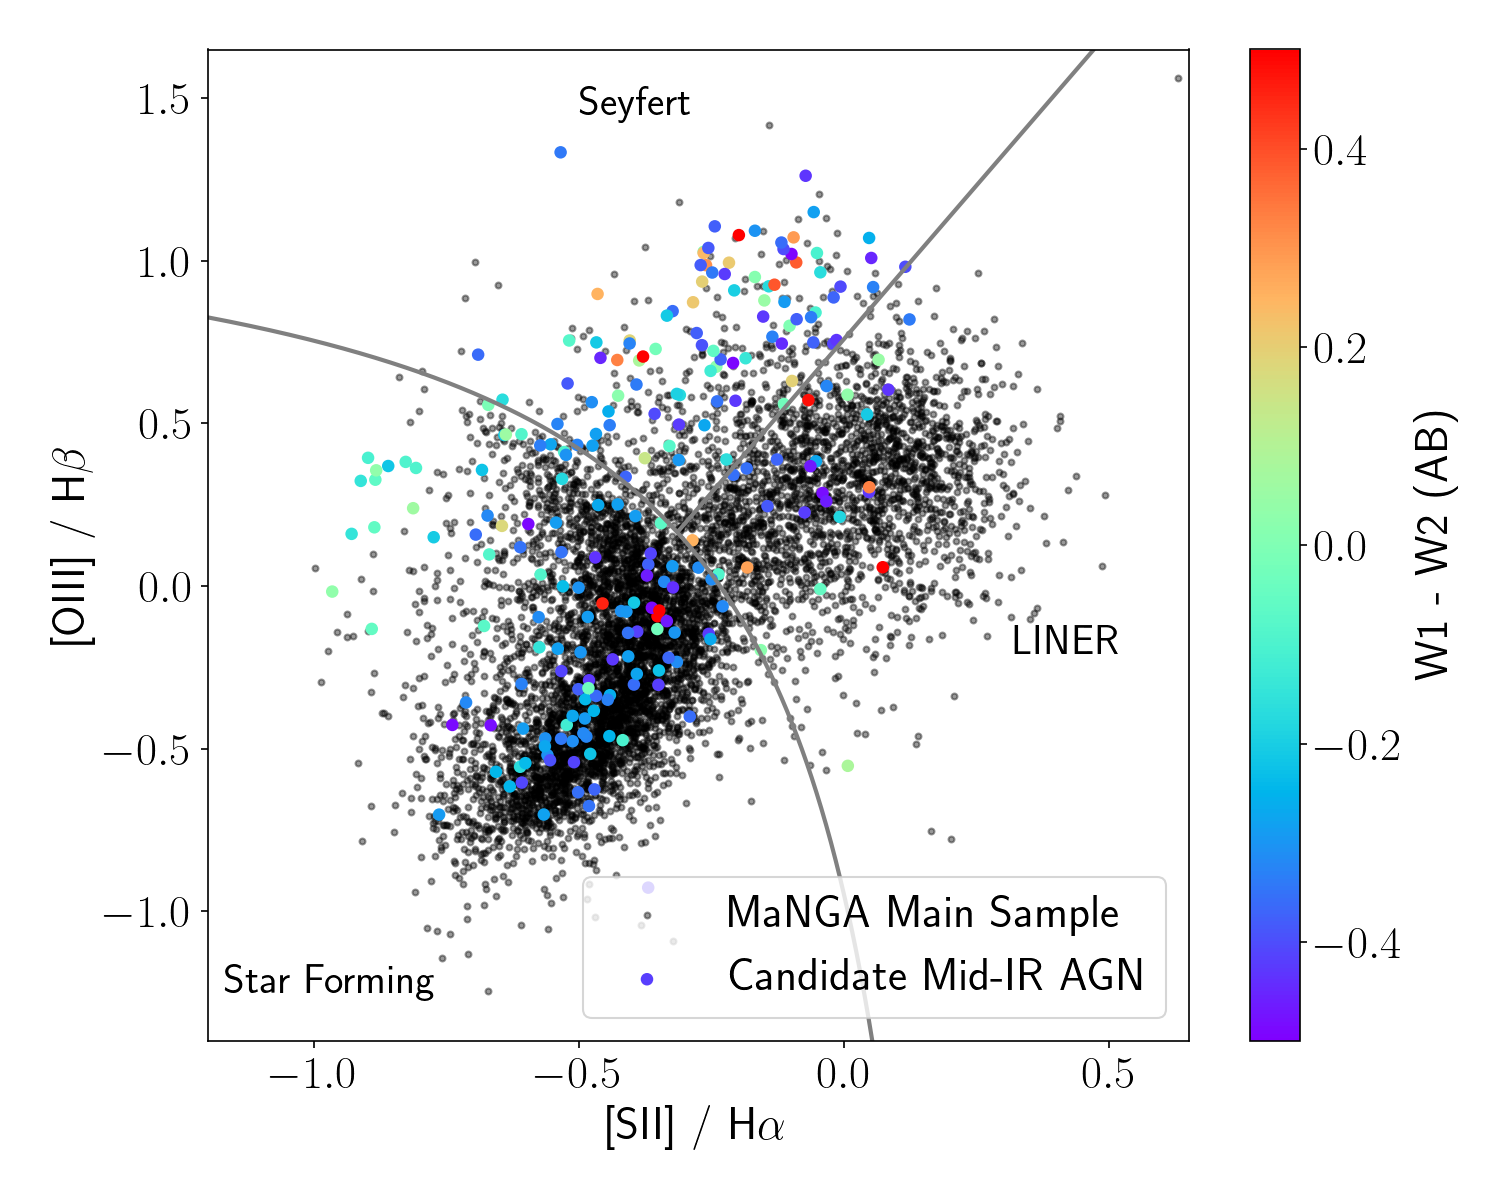
\includegraphics[width=0.91\textwidth]{bpt-agn.png}
\end{center}
\caption{\label{fig:bpt} The [SII]-based line ratio diagram
  \cite{veilleux87a} with standard divisions into ionization source
  classes: star formation, LINER, and Seyfert \cite{kewley06a}.  We
  expect that essentially all AGN with substantial hot dust emission
  will also have an ionized narrow line region, whose emission line
  ratios would be in the Seyfert region of this diagram if there was
  not competing emission from other components of the galaxy. Of all
  of our candidates, only about half have Seyfert classifications; the
  same is true for the more conservative mid-IR criterion of
  \cite{assef18a}. For ones without a Seyfert classification, although
  it is possible that the mid-IR colors may not be driven by an AGN,
  it also may be that the AGN narrow line emission may be outshown by
  star formation, which can easily happen at low Eddington ratios or
  high star formation rates \cite{trump15a}.  In short, the optical
  line ratio diagnostics cannot answer the central question posed by
  this proposal---motivating the proposed direct measurements of the
  mid-IR spectrum for these targets.  {\bf TODO: remove JWST}}
\end{figure}

\section{Objections, Uncertainties, Difficulties, and Their Mitigation}
\label{sec:difficulties}

The essential sources of uncertainty in our planned measurements
involve the validity of our W1$-$W2 selection criterion and our
ability to infer 6 $\mu$m AGN luminosity when there is significant
contaminating flux from stellar processes. If our planned measurements
are secure, variations among the population of mid-IR-emitting AGN can
complicate our interpretation (e.g. systematic differences in the AGN
mid-IR SED that cause selection effects that we do not model
successfully). In this section we describe these difficulties and how
we plan to diagnose and address them.

\noindent{\bf Why look in the mid-IR?} The mid-IR provides a unique
view of the population of AGN, in particular relative to the X-rays
and optical detection. It reveals obscured AGN whose emission is not
evident at other bandpasses. In addition, the mid-IR-emitting AGN
present promising targets for follow-up observations, since mid-IR
spectroscopy and time variability can yield important diagnostics of
the gas and dust structures deep inside the galactic nuclei. However,
rather than make a special case for the mid-IR instead of other
wavelength ranges, the key is that there is so much variation among
AGN manifestations that no single window onto their activity is
sufficient. We seek to understand the mid-IR {\it as part of} a
broader attack on local AGN demographics.

\noindent{\bf Are the AGN candidates actually AGN?} Our criterion for
selecting AGN from W1$-$W2 includes much bluer colors than even the
most inclusive color cuts used by others (e.g. from \cite{assef18a}).
We need to consider whether there are non-AGN SEDs that can explain
W1$-$W2 colors that are somewhat offset to the red relative to most
galaxies.  Low metallicity star burst components of the host galaxy
can redden the W1$-$W2 color across our threshold; for example,
\cite{hainline16a} argue that the W1$-$W2 color for starburst dwarf
galaxies can exceed even the more conservative criteria of
\cite{stern12a}.  Alternatively, in galaxies with intermediate age
stellar populations but little recent star formation, hot dust
envelopes of asymptotic giant branch stars can contribute to the W2
band and again lead to redder W1$-$W2 \cite{villaume15a}. For our
sample, with stellar masses mostly $> 10^9$ $M_\odot$ and redshifts
$z<0.15$, these issues are not particularly likely. We can use the
Spitzer spectra to diagnose these effects, and we can use the detailed
stellar population and emission line analysis of the optical MaNGA
spectra to characterize metallicities and star formation histories.
We admit that embarking on this study entails some risk, but if that
risk is realized, it may itself open up new scientific discoveries
about star formation and the interstellar medium of galaxies by
finding a particularly unusual type of galaxy.

\noindent{\bf Can we measure AGN luminosities accurately?} 
With a stringent cut on W1$-$W2, one can impute the majority of 
the W2 luminosity to the AGN emission. However, because we are
considering small offsets of a few tags of magnitudes from the 
``normal'' galaxies W1$-$W2 colors, our inference of the AGN-related
mid-IR luminosity is more uncertain. In Section \ref{sec:methods},
we describe two methods of estimating these luminosities, and comparisons
of these two methods will be used to assess how well we can recover
the AGN-related mid-IR luminosity. We will also explore the 
sensitivity of the estimates to the AGN SED model choices. 
We will use the Spitzer spectra to compare detailed fits to
those spectra to inferences from the broad-band photometry that we 
have for most of our sample. A reality check will be to compare
the 6 $\mu$m AGN-related luminosity to the [OIII] luminosity; these
two measures should correlate well in general, and we will 
examine outliers to assess whether they reveal failings in our
SED fitting or are truly interesting objects (or both).

\noindent{\bf Is our model for selection effects sufficiently good?}
For the inference of Eddington ratio distributions, we need to 
accurately understand the selection effects on detecting AGN. But 
if the mid-IR emission SED changes systematically with Eddington ratio
or galaxy host properties in the range we are studying, our model
of selection effects needs to account for this. For example, the
dust temperature distribution (which is plausibly related to Eddington 
ratio  and gas metallicity) changes the mid-IR emission spectrum.
Although to a limited degree we can use the Spitzer spectra to 
explore this variation, we will have consider variations in the
AGN SED used in the selection effect model, and evaluate the effect
of this uncertainty on our Eddington ratio distribution conclusions.

\noindent{\bf Isn't there a lot of complicated variation among AGN we
  are ignoring?}

\section{Project Plan and Timeline\label{sec:plan}}

The bulk of this work will be performed by a Graduate Research
Assistant (GRA) as their PhD thesis.  The PI will mentor the GRA and 
assist in data analysis, writing, and interpretation. An undergraduate
researcher will also assist in data analysis and data vetting.

\begin{ditemize}
\item {\it Year 1}: 
\begin{ditemize}
\item Develop AGN and galaxy SED fitting to determining 6 $\mu$ AGN luminosities and
upper limits from the WISE data.
\item Use Spitzer spectra to refine classification criteria, and to tune SED 
templates for accurately determining of 6 $\mu$m AGN luminosities and upper limits.
\item Publish catalog of AGN luminosities and upper limits, and methodology paper
on fitting AGN and galaxy SEDs.
\end{ditemize}
\item {\it Year 2}: 
\begin{ditemize}
\item Fit Eddington ratio distribution models 
using mid-IR AGN luminosities and upper limits.
\item Publish inferred  Eddington ratio distributions as a function of 
host galaxy stellar mass and SFR.
\item Publish comparison of mid-IR luminosities to other narrow-line,
radio continuum, and X-ray luminosities where available.
\end{ditemize}
\end{ditemize}

\section{Open Science and Data Management Plan\label{sec:data}}
\vspace{-6pt}

The data products will be WISE band luminosities and uncertainties, 
AGN classifications, AGN 6 $\mu$m luminosities, uncertainties, and 
upper limits, and SED fitting results for all 10,000 MaNGA galaxies. 
We will also produce SED fitting  to the Spitzer spectra used. These 
data will be stored as FITS files and distributed publicly.
We will submit them to SDSS to publish as a Value Added Catalog in a 
future data release.

The software pipeline will be version controlled using {\tt git} 
and distributed in a GitHub repository.
It will be licensed under the 3-clause Berkeley
Software Distribution (BSD-3) license.

\clearpage
\section{References}\label{sec:refs}

\printbibliography[title=~]

\clearpage
\section{Budget Narrative}\label{sec:budget}

\noindent {\bf Senior Personnel:} The PI is requesting 1.0 month of
summer salary for each of the 2 years of the project.  The PI is
responsible for the overall management of the project. The PI will
supervise the GRA and undergraduate and will assist in the writing,
data analysis, and interpretation.

\noindent {\bf Other Personnel:} Graduate Research Assistant (GRA):
Funds are requested for 2 academic years (AY) plus 2 summers. The GRA
will develop the software and perform the analysis described in the
proposal. Undergraduate Research Assistant (UGRA): Funds are requested
for an hourly research position. The UGRA will work with the GRA and
assist in the data analysis and data vetting.

\noindent {\bf Fringe Benefits Rate:} A fringe benefits rate 
applies to the PI salary and the undergraduate student salary. % 31%

\noindent {\bf Capital Equipment:} Funds are requested in Year 1 for 
dedicated computer  servers with which to perform the analysis (\$5,000 each
for two Dell PowerEdge R7525 Servers, with 2 16-core processers with 128M 
of cache, 4 Tb of local disk,  and 64 Gb of memory).

\noindent {\bf Domestic Travel:} Funds are requested for attendance at
one domestic conference for the GRA in each year. We assume \$1500 for
a 4-day conference (\$200 for registration fee, \$500 for airfare,
\$150/night for lodging, and \$50/night per diem).

\noindent {\bf Foreign Travel:} Funds are requested for attendance at
one foreign conference for the GRA in each year. For each conference
we assume \$1500 for a 4-day conference (\$200 for registration fee,
\$500 for airfare, \$150/night for lodging, and \$50/night per diem).

\noindent {\bf Publications:} We anticipate two 10-page journal
articles each year. Based on prior experience with the AAS Journals,
the typical publication cost will be \$1500 per paper in 2023 dollars.

\noindent {\bf Other Direct Costs:}
Graduate students receive tuition remission. % charged at 37% of
                                % graduate student salary in lieu of
                                % fringe benefits

\noindent {\bf Rates:} Senior personnel salaries increase XX\%
annually, while OTPS costs increase YY\% per year. % XX = 4, YY = 2.5

\noindent {\bf Indirect Costs:} An indirect cost rate has been
negotiated with DHHS, agreement dated October 6, 2021.
%The agreed upon
%rate for Facilities and Administration costs (F\&A) is 61\% as of FY
%2024 and thereafter.
The MTDC base excludes capital equipment, tuition
remission, participant support costs, and subcontracts beyond the
first \$25,000. 

\clearpage
\section{Summary of Work Effort}\label{sec:effort}

%The work will be divided as described in the table below.

\begin{table}[h!]
\centering
\caption{Personnel and Work Effort (all project years)\label{table:effort}} 
%\caption{Table of Work Effort\label{table:effort}} 
\begin{tabular}{lccc}
\\
\hline
& {\bf Funded Effort} & {\bf Unfunded Effort} & {\bf Total Effort} \\
{\bf Role} & {\bf (months / year)} & {\bf (months / year)} 
& {\bf (months / year)} \\
\hline
\hline
PI & 1 & 0 & 1 \\
Graduate Student & 12 & 0 & 12 \\
Undergraduate Student & 2 & 0 & 2 \\
\hline
\end{tabular}
\end{table}

\clearpage
\section{Budget Details}
\label{sec:budget-details}

\noindent {\bf Senior Personnel:}\\
{\it excluded as requested}

\noindent {\bf \it Other Personnel:}\\
\noindent {\bf Graduate Research Assistant (GRA):}\\
{\it excluded as requested}

\noindent {\bf Fringe Benefits Rate:}\\
{\it excluded as requested}

\noindent {\bf Capital Equipment:}\\
Year 1: \$10,000\\
Year 2: \$0

\noindent {\bf Domestic Travel:}\\
Year 1: \$1,500\\
Year 2: \$1,538

\noindent {\bf Foreign Travel:}\\
Year 1: \$1,500\\
Year 2: \$1,538

\noindent {\bf Publications:}\\
Year 1: \$3,000\\
Year 2: \$3,075

\noindent {\bf Other Direct Costs (Tuition Remission):}\\
Year 1: \$16,238\\
Year 2: \$16,806

\noindent {\bf Indirect Costs:}\\
{\it excluded as requested}

\end{document}
